\NeedsTeXFormat{LaTeX2e}
\documentclass[12pt, a4paper]{book}

\usepackage[Lenny]{fncychap}
\usepackage{fancyhdr}
\usepackage[utf8]{inputenc}
\usepackage{subfig}
\usepackage{epsfig}
\usepackage{epstopdf}
\usepackage{caption}
\usepackage{graphicx}
\usepackage{keyval}
\usepackage{float}
\usepackage{listings}
\usepackage{color}
\usepackage{textcomp}
\usepackage{datetime}
\usepackage[numbers, sort&compress, comma]{natbib}

\usepackage{subeqnarray}
\usepackage{bbm}
\usepackage{longtable}
\usepackage{rotating}
\usepackage{psfrag}
\usepackage{pifont}
\usepackage{fancybox}
\usepackage{amsmath}
\usepackage{amsfonts}
\usepackage [linktocpage]{hyperref}
\usepackage{amssymb,amsfonts}
\usepackage{multirow}
\usepackage{booktabs}
\usepackage{longtable}
\usepackage{float}
\usepackage{array}
\usepackage[acronym, nopostdot, nonumberlist]{glossaries}
\newglossary[nlg]{notation}{not}{ntn}{Notation}

\setcounter{tocdepth}{3}
\setcounter{secnumdepth}{5}

\setlength{\topmargin}{-1.1cm}
\setlength{\parskip}{\baselineskip}
\setlength{\parskip}{0.3cm}
\setlength{\textwidth}{16.5cm}
\setlength{\evensidemargin}{-0.4cm}
\setlength{\oddsidemargin}{0.3cm}
\setlength{\headsep}{1.0cm}
\setlength{\headheight}{3ex}
\setlength{\footnotesep}{5mm}

\renewcommand{\labelitemi}{$\bullet$}
\renewcommand{\labelitemii}{$\diamond$}
\renewcommand{\labelitemiii}{$\cdot$}

\lhead[\fancyplain{}{\thepage}]{\fancyplain{}{\sl\nouppercase\rightmark}}
\rhead[\fancyplain{}{\sl\nouppercase\leftmark}]{\fancyplain{}{\thepage}}
\cfoot{}

\ChTitleVar{\sf\Huge}
\ChTitleAsIs

\newcommand{\clearemptydoublepage}
{\newpage{\pagestyle{empty}\cleardoublepage}}

\newcommand{\R}{\mathbb{R}}
\newcommand{\x}{\mathbf{x}}
\newcommand{\grad}{\hspace{-2mm}$\phantom{a}^{\circ}$}

\makeglossaries


\newglossaryentry{gls:set}{
  name=set,
  description={A collection of distinct objects}}


\newacronym{CITIC-UGR}{CITIC-UGR}{Research Centre for Information and Communications Technologies of the University of Granada}

\newacronym{IMUs}{IMUs}{inertial measurement units}

\newacronym{MIMUs}{MIMUs}{magnetic inertial measurement units}
\newglossaryentry{not:F}{
  type=notation,
  name={$\mathbf{f}$},
  description={Force vector, $\mathbf{f} \in \mathbb{R}^3$},
  sort={f}}
  
\newglossaryentry{not:B_v}{
  type=notation,
  name={$\mathbf{B}$},
  description={Control matrix that relates the control input to the state $\mathbf{x}$},
  sort={Ba}}
 
\newglossaryentry{not:m}{
  type=notation,
  name={$m$},
  description={Mass},
  sort={m}}
  
\newglossaryentry{not:sigma}{
  type=notation,
  name={$\sigma$},
  description={Standard deviation},
  sort={sigma}}
  
\newglossaryentry{not:sigma_2}{
  type=notation,
  name={$\sigma^2$},
  description={Variance},
  sort={sigma}}
  
\newglossaryentry{not:mu}{
  type=notation,
  name={$\mu$},
  description={Mean value of conditional probability density},
  sort={sigma}}
  
\newglossaryentry{not:n}{
  type=notation,
  name={$n$},
  description={Fixed discrete time, non-dimensional number, or number of iterations, applied to recursive algorithms},
  sort={n}}
  
\newglossaryentry{not:a}{
  type=notation,
  name={$\mathbf{a}$},
  description={Acceleration vector, $\mathbf{a} \in \mathbb{R}^3$},
  sort={a}}
  
\newglossaryentry{not:impulse}{
  type=notation,
  name={$h_0, h_1, h_2, \dots$},
  description={Impulse response of a linear discrete-time filter},
  sort={h}}
  
\newglossaryentry{not:input}{
  type=notation,
  name={$z(0), z(1), z(2), \dots$},
  description={Time series that serves as input to a linear discrete-time filter},
  sort={yaa}}
  
\newglossaryentry{not:desired_response}{
  type=notation,
  name={$d$},
  description={Desired filter response of a linear discrete-time filter},
  sort={d}}
  
\newglossaryentry{not:error_signal}{
  type=notation,
  name={$e$},
  description={Error signal of a linear discrete-time filter},
  sort={e}}
  
\newglossaryentry{not:t}{
  type=notation,
  name={$t$},
  description={Continuous time},
  sort={t}}

\newglossaryentry{not:x_v}{
  type=notation,
  name={$\mathbf{x}$},
  description={State vector of a linear dynamical system},
  sort={xb}}
  
\newglossaryentry{not:x}{
  type=notation,
  name={$x$},
  description={One-dimensional location},
  sort={x}}
  
\newglossaryentry{not:displacement}{
  type=notation,
  name={$\Delta x$},
  description={One-dimensional displacement in $x$-direction},
  sort={x}}
  
\newglossaryentry{not:x_hat}{
  type=notation,
  name={$\hat{x}$},
  description={Estimate of $x$},
  sort={xa}}
  
\newglossaryentry{not:w_v}{
  type=notation,
  name={$\mathbf{w}$},
  description={Process noise vector},
  sort={wa}}
  
\newglossaryentry{not:v}{
  type=notation,
  name={$\mathbf{v}$},
  description={Measurement noise vector},
  sort={v}}
  
\newglossaryentry{not:u}{
  type=notation,
  name={$u$},
  description={Nominal velocity},
  sort={u}}
  
\newglossaryentry{not:w}{
  type=notation,
  name={$w$},
  description={Noise term},
  sort={w}}

\newglossaryentry{not:x_hat_v}{
  type=notation,
  name={$\hat{\mathbf{x}}$},
  description={Estimate of the state vector of a linear dynamical system},
  sort={xd}}
  
\newglossaryentry{not:x_hat_minus}{
  type=notation,
  name={$\hat{\mathbf{x}}^-_k$},
  description={A priori estimate of $\hat{\mathbf{x}}$, conditioned on all prior measurements except the one at time $t_k$},
  sort={xe}}
  
\newglossaryentry{not:z}{
  type=notation,
  name={$\mathbf{z}$},
  description={Observation or measurement vector of a dynamical system},
  sort={zaa}}
  
\newglossaryentry{not:H}{
  type=notation,
  name={$\mathbf{H}$},
  description={Measurement sensitivity matrix defining the linear relationship between the state of the dynamical system and the measurements that can be made},
  sort={Ha}}
  
\newglossaryentry{not:K_v}{
  type=notation,
  name={$\mathbf{K}$},
  description={Kalman gain matrix},
  sort={Kaa}}
  
\newglossaryentry{not:K}{
  type=notation,
  name={$K$},
  description={Weighting factor},
  sort={Ka}}
  
 \newglossaryentry{not:k}{
  type=notation,
  name={$k$},
  description={Discrete time normalised to sampling interval, that is sample number, $k \in \mathbb{N}^0$},
  sort={k}}
  
\newglossaryentry{not:P}{
  type=notation,
  name={$\mathbf{P}$},
  description={Covariance matrix of state estimation uncertainty},
  sort={P}}
  
\newglossaryentry{not:Q}{
  type=notation,
  name={$\mathbf{Q}$},
  description={Covariance matrix of process noise in the system state dynamics},
  sort={Q}}
  
\newglossaryentry{not:R}{
  type=notation,
  name={$\mathbf{R}$},
  description={Covariance matrix of observational (measurement) uncertainty},
  sort={R}}
  
\newglossaryentry{not:phi}{
  type=notation,
  name={$\bm{\Phi}$},
  description={State transition matrix of a discrete linear dynamical system},
  sort={phiaa}}
  
\newglossaryentry{not:x_k}{
  type=notation,
  name={$\mathbf{x}_k$},
  description={The $k$th element of a sequence $\dots$, $\mathbf{x}_{k-1}$, $\mathbf{x}_k$, $\mathbf{x}_{k+1}, \dots$ of vectors},
  sort={xc}}
  
 \newglossaryentry{not:unit-delay}{
  type=notation,
  name={$z^{-1}$},
  description={Unit-delay},
  sort={za}}
  
\newglossaryentry{not:roll}{
  type=notation,
  name={$\phi$},
  description={Roll angle that determines the rotation around the $x$-axis},
  sort={phi}}
  
\newglossaryentry{not:pitch}{
  type=notation,
  name={$\theta$},
  description={Pitch angle that determines the rotation around the $y$-axis},
  sort={theta}}
  
\newglossaryentry{not:yaw}{
  type=notation,
  name={$\psi$},
  description={Yaw angle that determines the rotation around the $z$-axis},
  sort={psi}}

\newglossaryentry{not:navigation_frame}{
  type=notation,
  name={$x, y, z$},
  description={Axes of the fixed world frame},
  sort={xayaza}}
  
\newglossaryentry{not:body_frame}{
  type=notation,
  name={$X, Y, Z$},
  description={Axes of the moving body frame},
  sort={xayazb}}
  
\newglossaryentry{not:transformation_matrix}{
  type=notation,
  name={$\mathbf{T}$},
  description={Transformation matrix},
  sort={Ta}}
  
\newglossaryentry{not:transformation_matrix_bn}{
  type=notation,
  name={$\mathbf{C}_{bw}$},
  description={Transformation matrix transforming a position vector from the body frame to the world frame},
  sort={Cbn}}
  
\newglossaryentry{not:transformation_matrix_nb}{
  type=notation,
  name={$\mathbf{C}_{wb}$},
  description={Transformation matrix transforming a position vector from the world frame to the body frame},
  sort={Cnb}}
  
\newglossaryentry{not:omega}{
  type=notation,
  name={$\bm{\Omega}_{\mathbf{E} \rightarrow \mathbf{E}'}$},
  description={Function that transforms a position vector $\mathbf{p}$ in the vector space $\mathbf{E}$ into the vector $\mathbf{p}^{'}$ in the vector space $\mathbf{E}^{'}$},
  sort={Om}}
  
\newglossaryentry{not:position_vector}{
  type=notation,
  name={$\mathbf{p}$},
  description={Position vector in a three-dimensional vector space},
  sort={p}}
  
\newglossaryentry{not:phi_vec}{
  type=notation,
  name={$\bm{\phi}$},
  description={Functional denoting the \emph{non-linear} transition matrix function of a discrete dynamical system},
  sort={phia}}
  
\newglossaryentry{not:h_vec}{
  type=notation,
  name={$\mathbf{h}$},
  description={Functional denoting the \emph{non-linear} measurement matrix function of a discrete dynamical system},
  sort={h}}

\newglossaryentry{not:resonance_freq}{
  type=notation,
  name={$\Omega$},
  description={Resonance frequency},
  sort={Omega}}
  
\newglossaryentry{not:force_one_d}{
  type=notation,
  name={$F$},
  description={One-dimensional force},
  sort={f}}
  
\newglossaryentry{not:damping_c}{
  type=notation,
  name={$D$},
  description={Damping coefficient},
  sort={D}}
  
\newglossaryentry{not:amplitude}{
  type=notation,
  name={$a$},
  description={Amplitude of an oscillating mode},
  sort={a}}
  
\newglossaryentry{not:angular_v_scalar}{
  type=notation,
  name={$\omega$},
  description={Scalar angular velocity},
  sort={omega}}
  
\newglossaryentry{not:spring_constant}{
  type=notation,
  name={$k_x$},
  description={Spring constant along the $x$-axis},
  sort={kx}}
  
\newglossaryentry{not:gravity}{
  type=notation,
  name={$\mathbf{g}$},
  description={Gravity vector},
  sort={g}}
  
\newglossaryentry{not:angular_velocity}{
  type=notation,
  name={$\bm{\omega}$},
  description={Angular velocity, $\bm{\omega} \in \mathbb{R}^3$},
  sort={omega}}

\newglossaryentry{not:mass_velocity}{
  type=notation,
  name={$\mathbf{v}$},
  description={Mass velocity, $\mathbf{v} \in \mathbb{R}^3$},
  sort={va}}  
  
\newglossaryentry{not:orthonormal_basis}{
  type=notation,
  name={$\mathbf{E}$},
  description={Orthonormal basis $\{x, y, z\} \in \mathbb{R}^3$},
  sort={E}}  
  
\newglossaryentry{not:identity_matrix}{
  type=notation,
  name={$\mathbf{I}_n$},
  description={Identity matrix $\mathbf{I}_n \in \mathbb{R}^n$},
  sort={I}}  

\newglossaryentry{not:magnitude_gravity}{
  type=notation,
  name={$\|\mathbf{g}\|$},
  description={Magnitude of the gravity vector},
  sort={ga}}    
  
\newglossaryentry{not:sampling interval}{
  type=notation,
  name={$T_s$},
  description={Sampling period},
  sort={T}}    
  
    
    
\hypersetup{
  pdftitle    = {Titel},
  pdfsubject  = {Electrical Engineering},
  pdfauthor   = {Robin Weiß},
  pdfkeywords = {Bachelor Thesis} ,
  pdfcreator  = {pdflatex},
  pdfproducer = {LaTeX}
}

\begin{document}

	\frontmatter

	\begin{titlepage}
\label{ch:titlepage}

\begin{center}


\includegraphics[width=7cm]{images/universidad_de_granada.eps}
	\hfill
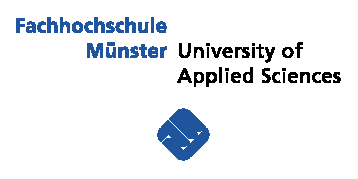
\includegraphics[width=5cm]{images/fh-muenster.eps} 

\vspace{2.5cm}

{\large \textsc{Münster University of Applied Sciences}}

Department of Electrical Engineering and Computer Science

\vspace{1.5cm}

{\large Bachelor Thesis}

\vspace{0.8cm}

\begin{LARGE}
\textsc{kalman filtering applied to orientation estimation in gait analysis}
\end{LARGE}

\vspace{1.8cm}

\begin{minipage}{0.4\textwidth}
\begin{flushleft}
\emph{Author:} \\
Robin Weiß
\end{flushleft}
\end{minipage}
\hfill
\begin{minipage}{0.5\textwidth}
\begin{flushright}
\emph{Supervisors:} \\
Prof. Dr.-Ing. Peter Glösekötter \\
Ph.D. Alberto Olivares Vicente \\
Prof. Dr. med. Kai Bötzel
\end{flushright}
\end{minipage}

\vspace{2.0cm}
	
\textit{A thesis submitted in partial fulfilment of the requirements for the degree\\
of Bachelor of Science in Electrical Engineering}

\vfill

\monthname \: \the\year 

\end{center}

\end{titlepage}

	\clearemptydoublepage
	
	\setcounter{page}{1}	
	\phantomsection
	\addcontentsline{toc}{chapter}{Statement of Authorship}
	\thispagestyle{empty}

\subsection*{Statement of Authorship}
I hereby certify that this bachelor thesis has been composed by myself, and describes my own work, unless otherwise acknowledged in the text. All references and verbatim extracts have been quoted, and all sources of information have been specifically acknowledged. It has not been accepted in any previous application for a degree.

\vspace{1cm}

\noindent 
Granada, $\the\day^{\text{th}}$ \monthname \: \the\year

\vspace{2cm}

\noindent
Robin Weiß

	\clearemptydoublepage
	
	\phantomsection
	\addcontentsline{toc}{chapter}{Preface}{\vspace{2em}}
	\chapter*{Preface}

This thesis entitled ``Analysis of anticipatory postural adjustments of Parkinson's patients using inertial sensors'' was submitted in partial fulfillment of the requirements for the degree of Bachelor of Science in Electrical Engineering awarded from the Münster University of Applied Sciences.

I took part in a conjoint project between the Research Centre for Information and Communications Technologies of the University of Granada (CITIC-UGR)\nomenclature{CITIC-UGR}{Research Centre for Information and Communications Technologies of the University of Granada} and the Department of Neurology of the Klinikum Großhadern in Munich, which is part of the Ludwig-Maximilians University. The objective of this thesis was to carry out an analysis of the so called anticipatory postural adjustments, which are the movements by a human subject between the moment he initiates gait and the first step.
	\clearemptydoublepage

	\phantomsection
	\addcontentsline{toc}{chapter}{Abstract}
	

\subsection*{Abstract}

This thesis entitled ``Analysis of anticipatory postural adjustments of Parkinson's patients using inertial sensors'' was submitted in partial fulfilment of the requirements for the degree of Bachelor of Science in Electrical Engineering. 

I took part in a conjoint project between the Research Centre for Information and Communications Technologies of the University of Granada (CITIC-UGR) and the Department of Neurology of the Klinikum Großhadern in Munich, which is part of the Ludwig-Maximilians University. The objective of this thesis was to carry out an analysis of the so called anticipatory postural adjustments, which are the movements by a human subject between the moment he initiates gait and the first step.

	\clearemptydoublepage
	
	\phantomsection
	\addcontentsline{toc}{chapter}{Contents}
	\tableofcontents
	\thispagestyle{plain}
		
	\listoffigures
	\phantomsection
	\addcontentsline{toc}{chapter}{List of Figures}
	\thispagestyle{plain}
	\clearemptydoublepage

	\listoftables
	\phantomsection
	\addcontentsline{toc}{chapter}{List of Tables}
	\thispagestyle{plain}
	\clearemptydoublepage	
	
	\printglossary[type=acronym, title={Abbreviations}]
	\phantomsection
	\addcontentsline{toc}{chapter}{Abbreviations}
	\thispagestyle{plain}
	\clearemptydoublepage
    
    \printglossary[type=notation]
    \phantomsection
    \addcontentsline{toc}{chapter}{Notation}
    \thispagestyle{plain}
    \clearemptydoublepage
	
	\mainmatter
	
	\pagestyle{fancyplain}
		
	\chapter{Introduction}
\label{ch:Introduction}

Monitoring and assessment of human body motion, in particular the analysis of gait, has become an integral part of medical diagnosis, therapy techniques, and rehabilitation \cite{tao_gait_2012}. \emph{Gait analysis} involves the measurement and assessment of quantitative parameters that characterise human locomotion. First research in this field was conducted in the late 19\textsuperscript{th} century \cite{tao_gait_2012}. The quantitative data enable physicians to diagnose a variety of medical conditions, validate treatment success, set goals in rehabilitation and regularly alter them when necessary. However, standard gait analysis based on multi-camera motion capture systems and force platforms require specialised gait laboratories, expensive equipment, and lengthy setup times. Moreover, the assessments of gait based on measurements performed in clinical settings might not be truly representative \cite{bonato_advances_2005}.

Unobtrusive wearable sensors mitigate the aforementioned limitations. Low cost sensors have been employed in clinical and home environments to constantly monitor the movements of patients \cite{godfrey_direct_2008}. The progressive miniaturisation of inertial and magnetic field sensors has made them more acceptable to patients and has consequently lead to an increasingly pervasive adoption for medical applications \cite{wee_soon_ambulatory_2008}, especially in the truly representative home environment.  Among others, wearable inertial and magnetic sensors are used to assess \emph{gait kinematics}. An extensive description is presented in Section \ref{sec:MARG_sensors_medical}. \emph{Kinematics} is a branch of classical mechanics, which is concerned with motion of objects without reference to the forces causing the motion. Position, velocity and acceleration are of particular interest in kinematics.

Determining the position of the legs is essential in gait analysis. The position, i.\,e. the orientation, can be estimated from inertial data. For the application in health care accurate orientation estimates are crucial. A high degree of precision based on data from miniaturised sensors necessitates adequate signal processing, in order to mitigate the influence of disruptive factors, such as bias instability and noise, among others. The signal processing of inertial and magnetic data encompasses calibration, adaptive filtering, and sensor fusion. The latter two are a part of this work.

\section{Motivation}

Gait analysis provides a powerful means to derive diagnostic information about the functioning of the musculoskeletal, vestibular, and central and peripheral nervous system \cite{bennett_extended_2013}. Accurate orientation estimation of the extremities by means of wearable inertial and magnetic field sensors allows objective assessment of human gait and can therefore benefit medical applications without the aforementioned constraints of camera based motion capture systems. A more reliable and more precise orientation estimation would enable an even more informative gait analysis. A multitude of applications in the medical field would profit from such an enhanced gait analysis \cite{wong_clinical_2007}. The direct relation to health care and the resulting possibility to improve the quality of life of many patients was the motivation for this thesis.

\section{Goals}

The goal of this thesis was implementing a new Kalman filter based orientation algorithm proposed by \citeauthor{bennett_motion_2014} in \cite{bennett_motion_2014}. Thus the estimation of orientation angles of the human leg by means of inertial and magnetic sensors should be improved. The filter algorithm should be implemented using \textsc{Matlab}\textsuperscript{\textregistered} and validated against existing algorithms by comparing their respective \gls{RMSE}. An existing system for human body motion analysis based on wearable sensors was available, so that no new hardware had to be developed to gather the movement data. A detailed description of the so-called GaitWatch system is found at the end of Chapter \ref{ch:MARG}.

\section{Methodology}

This document presents my work within the overall project in a chronological order. Subsequent to the previous introductory overview of the topic and the definition of the project objectives, this chapter ends with a description of the state of the art. To accomplish the tasks defined in the previous section, I had to acquire knowledge regarding various subjects. Chapters 2 to 4 outline the necessary fundamentals of MARG sensors, orientation estimation and digital filters, respectively.  This enables comprehension of the overall project, even for readers that are not familiar with some of the subjects. Those readers are referred to Chapters 2 to 4 at this point, before reading the state of the art. The actual implementation of the Kalman filter, including a prior theoretical design is given in Chapter 5. This chapter also encompasses the experimental setup, the results and a discussion of the latter. Finally, Chapter 6 covers conclusions and future work.

I implemented the filter algorithm in the numerical computing environment \textsc{Matlab}\textsuperscript{\textregistered}. As additional means to communicate with my supervisor and in order to enable him to follow the progress of my work at any time we used Pivotal Tracker, a tool for agile project management, and GitHub, a repository hosting service based on the distributed version control system Git. This thesis was written in \LaTeX{}.
 
\section{State of the Art}\label{sec:state_of_the_art}

There are several research works in the literature dealing with orientation estimation by means of inertial sensors. Kalman filters have been used successfully to improve the estimation of orientation angles from inertial data. The state of the art at the commencement of the project is described below. Subsequently, applications of wearable inertial sensors in health care and current attempts to revolutionise medical research assisted by those sensors are presented.

\subsection{Kalman Filtering in Orientation Estimation} \label{sec:state_of_the_art_kalman}

Considering the fact that inertial and magnetic field sensors are used to establish objective body motion parameters that affect medical diagnosis, therapy, and rehabilitation, the necessity of a high level of accuracy becomes obvious. In order to obtain precise orientation estimates from sensor data it is essential to mitigate the effects of measurement noise and to combine the advantages of different  sensors through sensor fusion. Therefore, a wide variety of Kalman filter algorithms have been developed in the literature. It is common practice to fuse accelerometer and gyroscope measurements to mitigate their respective drawbacks and thus obtain more accurate orientation estimates.

\citeauthor{Luinge_orientation_acc_gyro_99} \cite{Luinge_orientation_acc_gyro_99} alleged that the gravitational component of the acceleration signal has a greater magnitude than the component caused by motion for many human movements. They estimated the tilt angle, which is defined as the angle between the sensor axes and the vertical. The separate estimates from an accelerometer and a gyroscopes were fused with a Kalman filter. To test their method they moved the sensors around by hand for 30 seconds and then put it in a known position. They orientation obtained by integrating the angular rate only served as a reference. They concluded that a fusion of accelerometer and gyroscope signals accounts for a considerable improvement of the orientation estimation. This approach lacks of dynamical comparison since it only compares the errors at specific static positions.

Due to human motion intensity usually being subject to change, \citeauthor{olivares_vicente_signal_2013} implemented a \emph{gated Kalman filter} in \cite{olivares_vicente_signal_2013}. They modelled linear acceleration during intense motion as noise and improved the performance of the Kalman filter by dynamically adjusting the variance of both the process and measurement noise, according to the motion intensity. Therefore, they applied a \gls{LTSD} and set the variance between two predefined values. Then, the gated Kalman filter fused information from the accelerometer and the gyroscope signals. With this method they improved the adapting capability of the filter and consequently the precision of the orientation estimation.

\citeauthor{bennett_motion_2014} demonstrated in \cite{bennett_motion_2014} that accelerometer angle estimates are inaccurate for typical motions of the leg. They affirmed the need to decouple the acceleration due to motion from the acceleration due to gravity, since the former cannot be neglected during fast motions. Therefore, they deployed a \emph{kinematic model} of the leg to determine the acceleration that occurs due to motion and corrected the acceleration signal accordingly. An extended Kalman filter fused the corrected acceleration data with measurements of a gyroscope. This method improved upon the raw acceleration method during motion and at rest by an 83\% smaller \gls{RMSE}. Their proposed approach is the foundation of the filter algorithm implemented in Section \ref{sec:theoretical_design}.

\subsection{Wearable Sensors in Health Care}\label{sec:MARG_sensors_medical}

Inertial sensors can be found in smart phones, fitness trackers, and other wearable devices, among others. With increasing capability of body sensor networks and wearable computing, they have become prevalent in research environments for estimation and tracking of human body motion \cite{bennett_motion_2014}. They are used in activity monitoring \cite{veltink_detection_96, najafi_ambulatory_03, ermes_sports_08}, rehabilitation \cite{giggins_rehabilitation_13, lupinski_ligament_11}, sports training \cite{bonnet_squat_13, ermes_sports_08}, and localisation \cite{hoflinger_localization_13, Bennett_distance_13}.

Many neurodegenerative diseases such as, for instance, Parkinson's disease, impair stable stance and gait and reduce the patient's mobility. Thus, they diminish the quality of life significantly. \emph{Parkinson's disease} is a movement disorder that is characterised by marked slow movements, tremors, and unstable posture. Especially in advanced stages of the disease many patients exhibit an episodic, brief inability to step, which delays gait initiation or interrupts ongoing gait. This phenomenon is called freezing of gait. With the progression of the disease, Parkinson's patients are increasingly dependent on help from others to accomplish daily tasks. One of the most reliable diagnostic criterion of the disease is gait \cite{tao_gait_2012}. Hence, wearable motion sensors have been used successfully to classify the severity of the disease objectively \cite{mancini_anticipatory_2009, palmerini_feature_2011, klerk_long-term_2009}.

Stroke patients, who regained their walking ability, need to undergo rehabilitation to recover their independent mobility. Ambulatory gait analysis provides a means to assess the function of the lower extremities of hemiparetic post-stroke patients and follow the progress of rehabilitation \cite{tao_gait_2012, saremi_reliability_2006}. In addition, the presence of neurologic gait abnormalities is used as a significant predictor of the risk of development of dementia \cite{verghese_dementia_2002}. Also, emergency falls of elderly people can be detected \cite{bourke_threshold-based_2008, bourke_assessment-waist_2010, bourke_fall_detection_2008}.

\subsection{The Impact of Wearable Sensors on Medical Research}

The fact that most of the current smartphones come equipped with inertial and magnetic sensors and powerful processor has opened up new possibilities for medical research. The number of smartphones across the globe is predicted to surpass two billion in 2016 \cite{emarketer_smartphones}. Recently, large companies have developed software that takes advantage of the associated potential to revolutionise medical research.

In August 2014, the Michael J. Fox Foundation for Parkinson’s Research and Intel Corporation \cite{Intel_2013} announced a collaborative research study on objective measurement of Parkinson symptoms. They aim to collect movement data of thousands of patients twenty-four seven at over 300 samples per second by means of unobtrusive wearable devices and store them on a big data analytics platform. The data platform, deployed on a cloud infrastructure, supports an analytics application that processes the data and detects changes in real time. Thus, by detecting anomalies, the progression of the disease can be measured objectively without the need for scientists to focus on the underlying computing technologies. Physicians and researchers are intended to have access to the data as well as be able to submit their own anonymised patient data for analysis. According to \cite{Intel_2013} the correlation of data that quantifies symptoms such as slowness of movement, tremor, and sleep quality with molecular data could advance drug development and provide a deeper insight into the clinical course of Parkinson's disease.

In March 2015, \citeauthor{Apple_2015} announced a platform-independent, open source software framework called ResearchKit \cite{Apple_2015} that, amongst others, takes advantage of the MARG sensors in the iPhone to track movement of patients in daily life. Thus medical researchers obtain robust data with far more regularity than it was possible when patients complete tasks at hospitals or other research facilities in irregularly intervals. Moreover, according to \citeauthor{Apple_2015} ResearchKit simplifies recruiting participants from all over the world, which results in a more varied study group that provides a more useful representation of the population. Together with the University of Rochester and Sage Bionetworks they announced the iPhone app `mPower' \cite{mpower}, which measures balance and gait of Parkinson patients to help researchers better understand how various symptoms are connected to Parkinson's disease.


	\chapter{Hardware Description}
\label{ch:Hardware}
Along this chapter we will introduce a general description of all devices used to data gathering for the development of this project.


It should be noted at this point that there are two clearly differentiated parts. In the first of them, we work with Force Plate and GaitWatch data, taking out their characteristic signals and synchronising them. In the second of them, we work jointly with Gait Watch and Qualisys System data for the purpose of comparing the accuracy in the calculated orientation angles.


\section{GaitWatch}

GaitWatch is an Inertial Measurement Unit (IMU) designed for gait monitoring of patients. It was developed by Prof. Dr. Med. Kai Bötzel at the Department of Neurology of Ludwig-Maximilians University in Munich in conjunction with Dr. Alberto Olivares Vicente from the Department of Signal Theory, Telematics and Communications of the University of Granada \cite{OlivaresBotzel2013}.

The system is composed of the central processing unit and
a set of measuring units which are wired to it. The measuring units are 
placed in the patients’ thighs, shanks, arms and trunk.

\begin{figure}[H]
	\centering
	\epsfig{file=imagenes/GeneralDiagramGW, width=7cm}
	\caption{General Diagram of the Gait Watch.}
	\label{fig:diagram}
\end{figure}

The central processing unit has a microcontroller is in charge of gathering the data from the external measurement units and writing it to the memory card. So, this central unit is placed in the trunk inside a box and it contains an AL-XAVRB board with an AVRATxmega processor which contains the necessary embedded firmware to gather the data from all the measurement units and store it in a microSD card. Also, the trunk box contains some embedded magnetic and inertial sensors.

\begin{figure}[H]
	\centering
	\epsfig{file=imagenes/devicesGW, width=7cm}
	\caption{Devices used in Gait Watch System.}
	\label{fig:devicesGW}
\end{figure}

There are three different kinds of external units with the following components:
\begin{itemize}
	\item Type A (thighs and shanks): 
	\begin{itemize}
		\item IMU 5 from Sparkfun. IMU 5 contains an IDG500  biaxial gyroscope (from which only Y axis is actually used) with a measurement range of $\pm500deg/s$ and a $\pm3g$ triaxial accelerometer, ADXL335 .
	\end{itemize}
	\item Type B (arms):
	\begin{itemize}
		\item IDG500  biaxial $\pm500deg/s$ gyroscope.
	\end{itemize}
	\item Type C (trunk box):
	\begin{itemize}
		\item ADXL345  triaxial accelerometer with programmable range ($\pm16g/\pm8g/\pm4g/\pm2g$).
		\item IMU3000 triaxial gyroscope with programmable range ($\pm250/\pm500/\pm1000/\pm3000 (deg/s)$).
		\item Micromag3  triaxial magnetometer ($\pm11Gauss$).
	\end{itemize}
\end{itemize}


\section{Force Platform}
Force Plate (FDM-S Multifunction Force-measuring Plate, Zebris) is a System for force measurement and it can be used as a complete measuring unit for stance and roll-off analysis \cite{forceplate}.

This platform consist of a large number of force sensors and enables the distribution of static and dynamic forces under the feet to be analyzed during stance and gait (65x40 cells of sensors). As a result, foot deformities, foot function and posture can be analysed and are available as an evaluation report \cite{forceplate}.

Therefore, this gathered information can be used afterward to analyse the postural adjustments with the right software.

\begin{figure}[H]
	\centering
	\epsfig{file=imagenes/FDMS_Zebris, width=7cm}
	\caption{Platform used to analyse the force under the feet.}
	\label{fig:FDMS}
\end{figure}


\section{Qualisys System}
The Qualisys optical motion tracker is a system that uses high speed digital cameras to capture the motion of a measurement object with passive or active markers attached \cite{OlivaresBotzel2013}.

This technology is used by researchers and clinicians to undertand the basic for human motion or improve treatment during a reabilitation process. Also, it used in industrial applications, for example, the interior design of a car can be improved by using this System to evaluate the confort and safety factors for the car driver \cite{Qualisys}.

The technology is precise and delivers high quality data to the observer in real-time. The core component of Qualisys System is one or more infrared optical cameras that emit a beam of infrared light. Also, there are small retro-reflective markers on a object or person. When the cameras emit infrared light onto the markers, these reflect the light back to the camera sensor and this information is used to calculate the position with high spatial resolution  \cite{Qualisys}. The used system has eight cameras which are distributed around a room.

\begin{figure}[H]
	\centering
	\epsfig{file=imagenes/QualysisSystem, width=7cm}
	\caption{Qualisys optical motion tracker.}
	\label{fig:QS}
\end{figure}

The provided software tools allows to perform basic motion calculations,
such as speed, acceleration, rotation and angle, as well as other more complex
calculations. The precision of this system allows its use as a reference system to evaluate portable motion tracking systems such as the GaitWatch  \cite{OlivaresBotzel2013}.

	\chapter{Results and Discussion}
\label{ch:Results and Discussion}


	\chapter{Conclusion and Future Work}
\label{ch:Conclusion and Future Work}

\section{Conclusions}

Gait analysis is a useful tool both in clinical practice and biomechanical research. In this work I implemented an extended Kalman filter along with some auxiliary routines that . and showed that motion-based acceleration correction can improve the angle estimates during faster motion. In order to replace a camera-based motion capture system with low cost wearable MARG sensors, some technical deails need to be improved. One could use a more complex mathematical model of the leg that takes motions outside 

Summarising the above, I can say that I have learned a lot in the four month that I spent in Granada. Amongst others I have come to know many new work methods, not only due to being exposed to people from a different culture, but also due to the fact that scientific research differs strongly from the work as a student at university. I gained a deeper understanding of orientation estimation and how Kalman filtering  benefits the accuracy. I improved my MATLAB$\textsuperscript{\textregistered}$ skills and I am now familiar with tools such as GitHub and Pivotal Tracker which make working in a team much easier and significantly more efficient.  While working at the research centre, I obtained a valuable insight into scientific research and could improve my oral and written English skills. Furthermore I now know the fundamentals of \LaTeX{}.

All in all it was a great experience, professionally as well as personally. I truly and unreservedly recommend such a stay to \emph{every} university student.

\section{Future Work}

%Medical engineering is a very interesting blend of both my major interests, that is, working in the medical field as a paramedic and  in the technical field as an electrical engineer. There is a variety of possible future work. One related topic would be the validation of the pitch angles measured with the gyroscopes of the GaitWatch by means of cameras that record the trace of visual markers. From these markers one could compute the pitch angels and compare them to the those of the GaitWatch.



	
	\clearemptydoublepage
	\bibliographystyle{unsrtnat}
	\addcontentsline{toc}{chapter}{Bibliography}
	\bibliography{Bibliography}
	
	\clearemptydoublepage
	
\end{document}
